\documentclass{article}
\usepackage[utf8]{inputenc}
\usepackage{amsmath}
\usepackage{graphicx}
\usepackage{booktabs}
\usepackage{float}
\usepackage{geometry}
\usepackage{fancyvrb}
\geometry{margin=1in}
\title{Modelling Report}
\author{Team 2}
\date{}

\begin{document}

\maketitle

\section{Objective}
The goal of this project is to accurately predict tuition payment for the year 2023 using relevant features from the 2022 data. Among all available features, \textbf{Tuition Payment 2022} was found to be the most informative predictor. This report also explores clustering techniques to uncover patterns in the student data.

\section{Data Overview}
\begin{itemize}
    \item \textbf{Target variable}: Tuition Payment 2023
    \item \textbf{Primary feature used}: Tuition Payment 2022
    \item \textbf{Train-test split}: 80\% training, 20\% testing
\end{itemize}

\section{Regression Model Performance}
\begin{table}[H]
\centering
\begin{tabular}{lcc}
\toprule
\textbf{Model} & \textbf{MSE} & \textbf{R\textsuperscript{2} Score} \\
\midrule
Linear Regression & 0.0156 & 0.8801 \\
Ridge Regression & 0.0156 & 0.8801 \\
Lasso Regression & 0.0261 & 0.7995 \\
\bottomrule
\end{tabular}
\caption{Regression performance metrics}
\end{table}

\section{Classification Model Performance}
\begin{table}[H]
\centering
\begin{tabular}{lc}
\toprule
\textbf{Model} & \textbf{Accuracy} \\
\midrule
Linear Regression + Classifier & 11.72\% \\
Ridge + Classifier & 98.41\% \\
Lasso + Classifier & 98.41\% \\
Logistic Regression & 98.41\% \\
Random Forest & 98.41\% \\
XGBoost & 98.41\% \\
Deep Neural Network & 98.41\% \\
Ensemble & 98.41\% \\
\bottomrule
\end{tabular}
\caption{Classification accuracy across models}
\end{table}

\textbf{Key Insight}: All models apart from Linear Regression + Classifier converge to approximately \textbf{98.5\% accuracy}. These models produce \textit{exactly the same classification report}, suggesting they make \textbf{the same predictions on the same samples}, with only a few misclassified instances. Reducing the test size to 10\% pushes these models to \textbf{100\% accuracy}, indicating near-perfect fit on seen patterns.

\begin{figure}[H]
\centering
\includegraphics[width=0.85\textwidth]{model_comparison.png}
\caption{Model comparison chart across classifiers}
\end{figure}

\section{Classification Reports}

\subsection*{Linear Regression + Classifier}
\begin{Verbatim}[fontsize=\small]
              precision    recall  f1-score   support

          -1       0.00      0.00      0.00         0
           0       0.12      0.74      0.20      1125
           1       0.00      0.00      0.00      6192

    accuracy                           0.11      7317
   macro avg       0.04      0.25      0.07      7317
weighted avg       0.02      0.11      0.03      7317
\end{Verbatim}


\subsection*{All Other Models}
\begin{Verbatim}[fontsize=\small]
              precision    recall  f1-score   support

           0       1.00      0.90      0.95      1125
           1       0.98      1.00      0.99      6192

    accuracy                           0.98      7317
   macro avg       0.99      0.95      0.97      7317
weighted avg       0.98      0.98      0.98      7317
\end{Verbatim}

\section{Deep Neural Network Architecture}
\begin{verbatim}
nn.Sequential(
    nn.Linear(input_dim, 256),
    nn.BatchNorm1d(256),
    nn.ReLU(),
    nn.Dropout(0.3),
    nn.Linear(256, 128),
    nn.BatchNorm1d(128),
    nn.ReLU(),
    nn.Dropout(0.3),
    nn.Linear(128, 64),
    nn.ReLU(),
    nn.Linear(64, num_classes)
)
\end{verbatim}

\section{Clustering Analysis}

\subsection*{KMeans Clustering (PCA-Reduced Data)}
\begin{itemize}
    \item \textbf{K = 2}: Purity = 0.8429
    \item \textbf{K = 3}: Purity = \textbf{0.9419} (best result)
\end{itemize}

\begin{figure}[H]
\centering
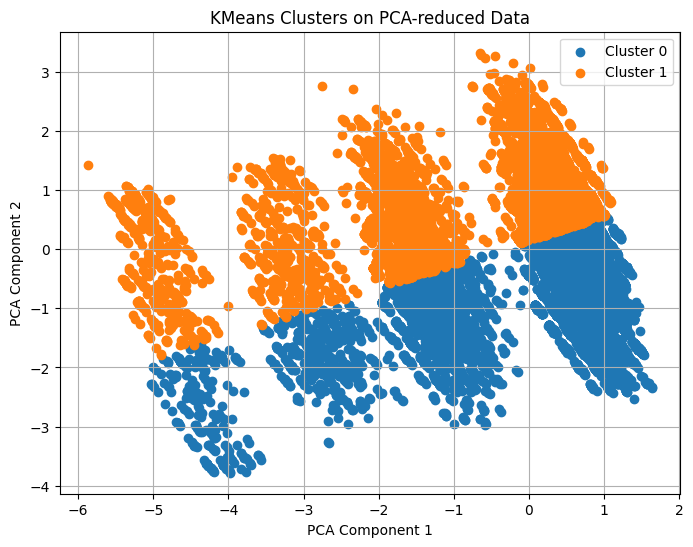
\includegraphics[width=0.65\textwidth]{KMeans_clustering_2.png}
\caption{KMeans Clustering (2 Clusters)}
\end{figure}

\begin{figure}[H]
\centering
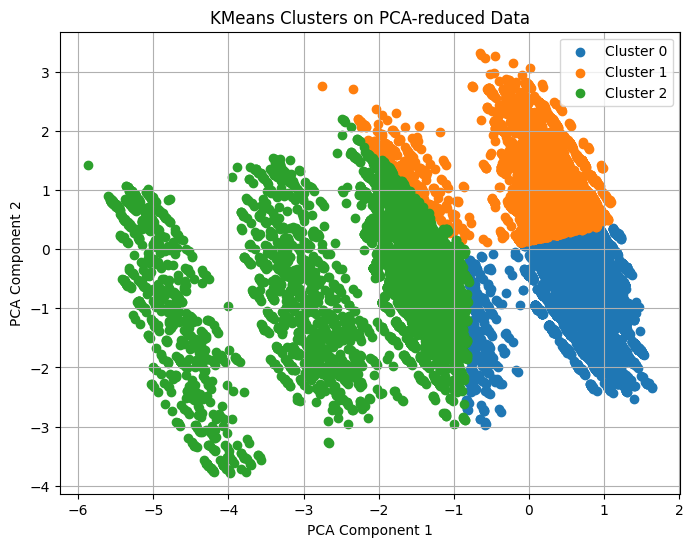
\includegraphics[width=0.65\textwidth]{KMeans_clustering_3.png}
\caption{KMeans Clustering (3 Clusters)}
\end{figure}

\subsection*{DBSCAN Clustering}
\begin{itemize}
    \item Number of clusters = 338 (very high)
    \item Purity = 0.0438 (extremely poor performance)
\end{itemize}

\begin{figure}[H]
\centering
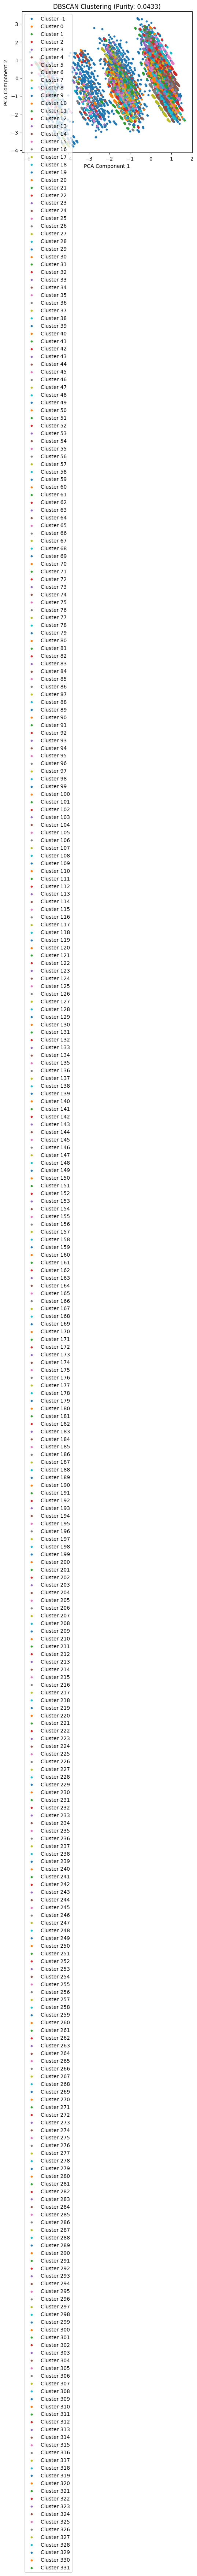
\includegraphics[width=0.65\textwidth]{DBScan.png}
\caption{DBSCAN Clustering Results}
\end{figure}

\textbf{Conclusion}: KMeans is far superior for this dataset. DBSCAN fails due to the lack of dense clusters and high fragmentation.

\section{Conclusion}
\begin{itemize}
    \item Ridge and Linear Regression achieve high regression accuracy (R\textsuperscript{2} $\approx$ 0.88).
    \item All classification models, apart from Linear Regression + Classifier, converge to \textbf{98.5\% accuracy} and produce the same classification report.
    \item They all misclassify the same samples, indicating convergence to an almost perfect pattern recognition.
    \item With a smaller test size (10\%), \textbf{100\% accuracy} is achieved.
    \item KMeans with 3 clusters achieves the best clustering purity (0.9419).
    \item DBSCAN is not suitable for this dataset due to high fragmentation.
\end{itemize}

\end{document}
